\chapter{Estudio sobre el Aluminio 1050 laminado simétricamente}\label{C:AlS}
\graphicspath{{./figs/06_Al/}}

En este capítulo se estudiará la microestructura de chapas aluminio, laminadas simétricamente.
El aluminio es un material FCC con alta energía de falla de apilamiento y capacidad de recristalizar dinámicamente[ref].
Las chapas fueron obtenidas comercialmente y son de la aleación 1050, lo que significa que se trata de aluminio con baja cantidad de aleantes, y con capacidad de ser endurecido por trabajado.
Estas aleaciones poseen elevada ductilidad, resistencia a la corrosión y buena soldabilidad.\cite{ESAB:AlAlloys,AlOrg:AlAlloys,PAInt:AlAlloys}.
En estas condiciones se espera que el material sea fácil de deformar, lo que en el caso del laminado significa que se pueden lograr elevadas reducciones incluso deformando a temperatura ambiente.
Los usos principales de este material son aquellos en que la resistencia a la corrosión son importante, como ser la industria química y la alimenticia\cite{PAInt:AlAlloys,AZOM:AlAlloys}.
Debido a la tendencia de este material a recristalizar dinámicamente, también se espera que se acumulen pocas dislocaciones, ya que las mismas se pueden limpiar por recristalizado dinámico inducido por la deformación aplicada.

Los análisis realizados utilizando el método CMWP en las chapas estudiadas dan un valor promedio de factor de Wilkens del orden de la unidad, lo que indica que se puede suponer que existe poca correlación en las dislocaciones acumuladas, lo que a su vez hace a este material apropiado para ser estudiado dentro del modelo de Langford.
En particular, se estudiarán chapas de aluminio que desarrollaron texturas diferentes como producto del laminado: una que desarrolló la textura típica de laminado de los materiales con estructura cristalina FCC, y otra que mantuvo la textura cúbica de partida.

\section{Análisis de la textura}\label{S:AlText}
En la Fig. \ref{fig:AlPDF} se pueden observar las figuras de polos recalculadas para los dos aluminios laminados simétricamente, donde puede apreciarse claramente que ambos materiales han desarrollado texturas completamente diferentes.

Las chapas comerciales de aluminio provienen de un tren de laminado en caliente, lo que hace que estos materiales tengan como textura de partida la textura de recristalizado, que en el caso del aluminio puro es la textura cúbica[ref].

Los dos aluminios se laminaron de la misma manera, con la misma cantidad de pasos?

Sin embargo, la laminación simétrica con reducciones del 70\,\% o más suele introducir suficiente deformación en el material como para destruir completamente la textura de partida del mismo.
La textura de laminado del aluminio se caracteriza principalmente por componentes que se encuentran presentes a lo largo de la denominada fibra $\beta$, que va desde la orientación Cu = \{112\}\textless 111\textgreater, pasando por la orientación S = \{123\}\textless 634\textgreater, hasta la orientación Bs = \{011\}\textless 211\textgreater\cite{jata2013aluminum,Hirsch19882863,Engler1996187}.
La textura típica de los procesos de laminado simétrico en materiales FCC produce figuras de polos como la que se observa en la Fig.\,\ref{fig:AlPDF}-b, en cuyo caso se dice que el material tiene una textura de laminado de tipo cobre\cite{kocks2000texture}. Sin embargo, en materiales que tienden a recristalizar dinámicamente, si la textura cúbica de partida es muy intensa, puede ocurrir que la textura de recristalizado permanezca incluso a altas deformaciones, que es lo que ocurrió con la chapa cuyas FPs se ve en la Fig. \ref{fig:AlPDF}-a donde aparte de una intensa textura cúbica se puede apreciar una fibra \{001\}\textless 100\textgreater de baja intensidad.

\begin{figure}[!htb]
  \centering
  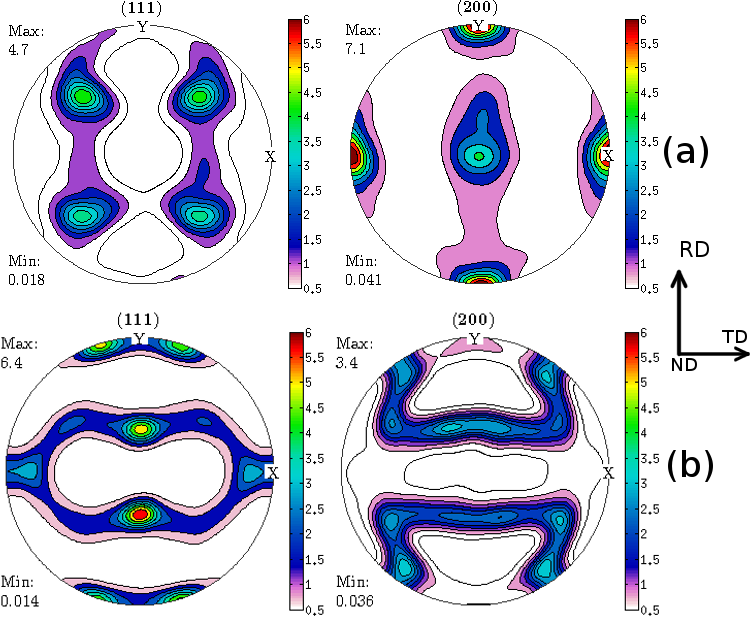
\includegraphics[width=0.8\textwidth]{AlText}
  \caption{Figuras de polos de dos chapas de aluminio 1050 laminadas hasta lograr una reducción del 70\,\%. En la Fig. (a) se puede apreciar que el aluminio conservó la textura cúbica de partida, mientras que en la (b) la chapa terminó adquiriendo la textura de laminado típica de un material FCC con alta energía de apilamiento.}
  \label{fig:AlPDF}
\end{figure}

La presencia de una textura cúbica o de laminado tipo cobre confirman la baja presencia de maclas y otro tipo de fallas de apilamiento en el material.
Como contraposición, el lector puede observar la textura de laminado del acero F138 en la Fig. \ref{fig:F138PF}, donde la presencia de aleantes ha bajado la energía de falla de apilamiento, lo que a su vez produce una textura de compresión con una fuerte presencia de la fibra \{110\}\textless 001\textgreater.
Cabe mencionar aquí también lo mencionado en el Cap. \ref{C:F138}, donde se mostró que la medición de la textura del acero F138 empleando rayos X de laboratorio mostró que el mismo exhibe la textura de laminado del latón, como era de esperarse.

En lo sucesivo, y para distinguir a ambos materiales, se denominará a la muestra que conservó la textura cúbica como $Al_C$, y a la muestra que desarrolló la textura de laminado como $Al_L$.

En la Fig. \ref{fig:AlODF} se pueden apreciar las secciones $\phi_2 \ = \ 0$\,$^{\circ}$ y $\phi_2 \ = \ 45$\,$^{\circ}$ de las muestras $Al_C$ (Fig. \ref{fig:AlODF}-a) y $Al_L$ (Fig. \ref{fig:AlODF}-b).

\begin{figure}[!htb]
  \centering
  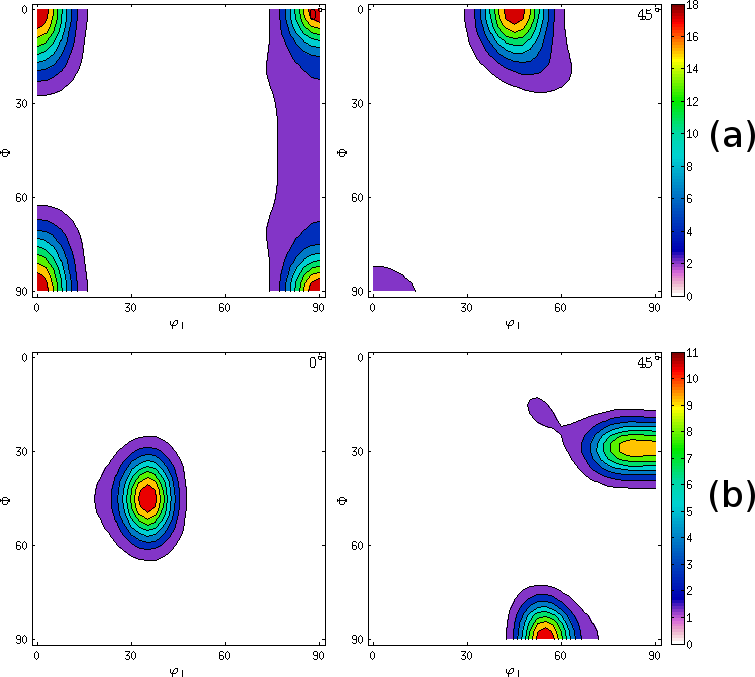
\includegraphics[width=0.8\textwidth]{AlODF}
  \caption{FDO de las chapas de aluminio. Al observar las secciones $\phi_2 \ = \ 0$\,$^{\circ}$ y $\phi_2 \ = \ 45$\,$^{\circ}$ puede apreciarse más claramente que la principal componente de la textura de $Al_C$ es la cúbica, con una pequeña componente de fibra \{001\}\textless 100\textgreater, mientras que la muestra $Al_L$ tiene las componentes que se esperan en un material FCC laminado, es decir, la componente Goss y la \ldots}
  \label{fig:AlODF}
\end{figure}

\newpage
\section{Estudio de la microestructura de la muestra $Al_C$ por el método de Langford y figuras de polos generalizadas}\label{S:AlCLANG}

\begin{figure}[!htb]
  \centering
  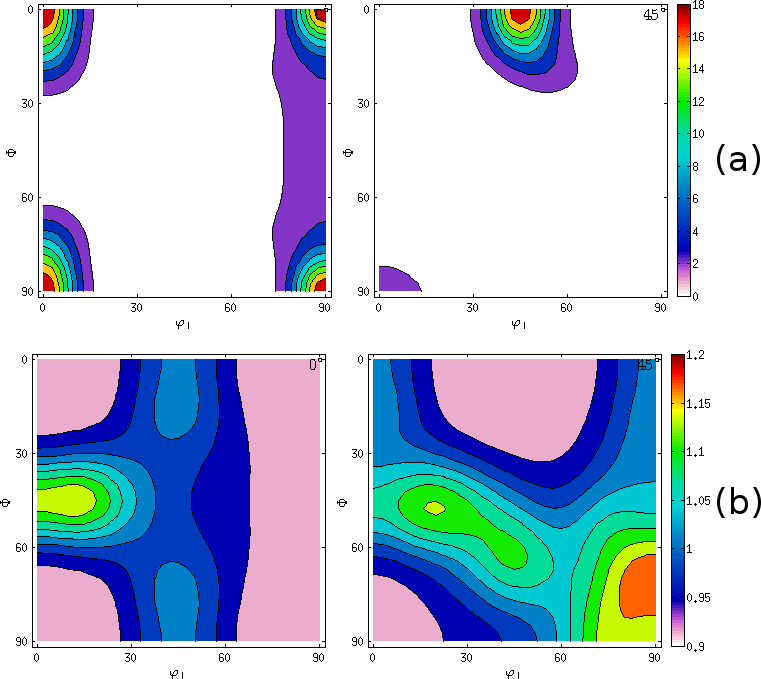
\includegraphics[width=\textwidth]{FWHMvsODF_AlC}
  \caption{FWHM vs ODF para $Al_C$.}
  \label{fig:AlCFWHMODF}
\end{figure}

\begin{figure}[!htb]
  \centering
  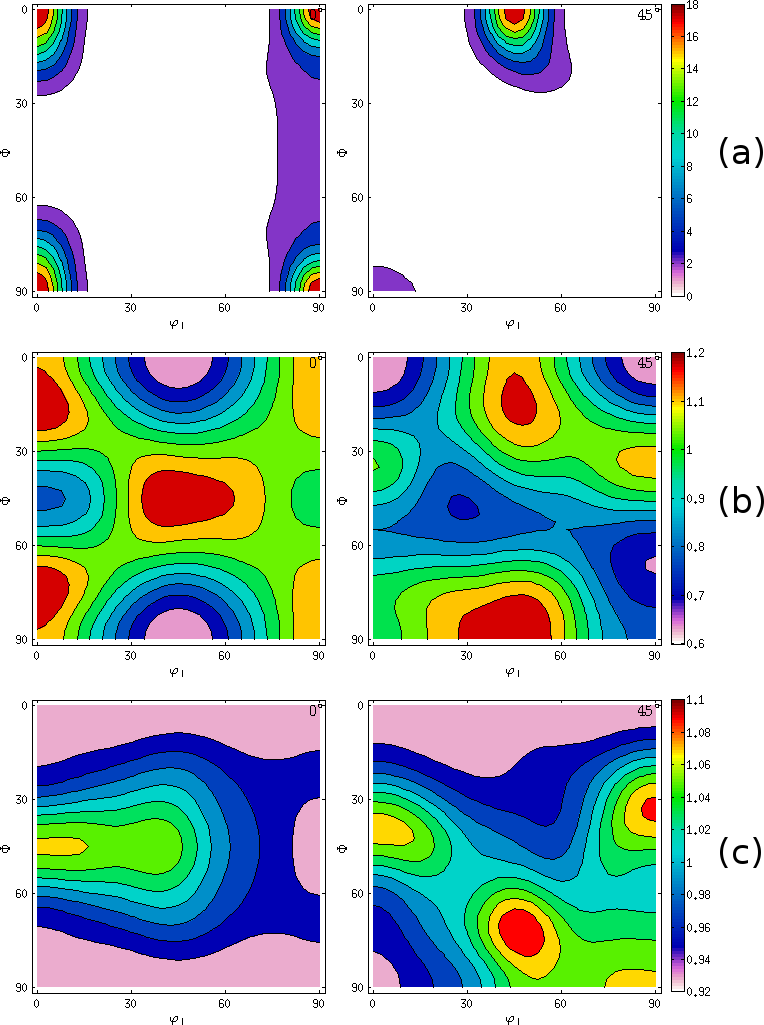
\includegraphics[width=\textwidth]{MicrovsODF_AlC}
  \caption{Size y strain vs ODF $Al_C$.}
  \label{fig:AlCMicro}
\end{figure}

\newpage
\section{Estudio de la microestructura de la muestra $Al_L$ por el método de Langford y figuras de polos generalizadas}\label{S:AlLLANG}
\begin{figure}[!htb]
  \centering
  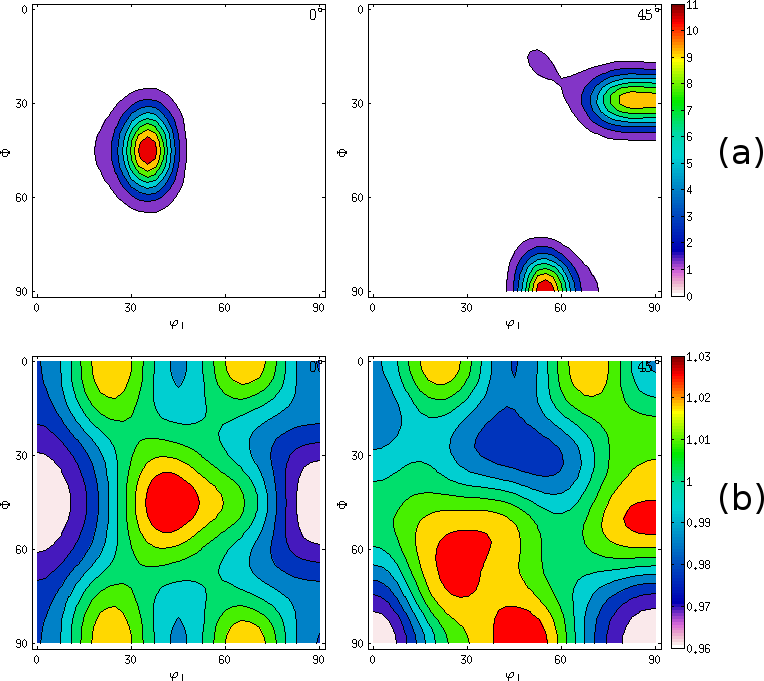
\includegraphics[width=\textwidth]{FWHMvsODF_AlL}
  \caption{FWHM vs ODF para $Al_L$.}
  \label{fig:AlLFWHMODF}
\end{figure}

\begin{figure}[!htb]
  \centering
  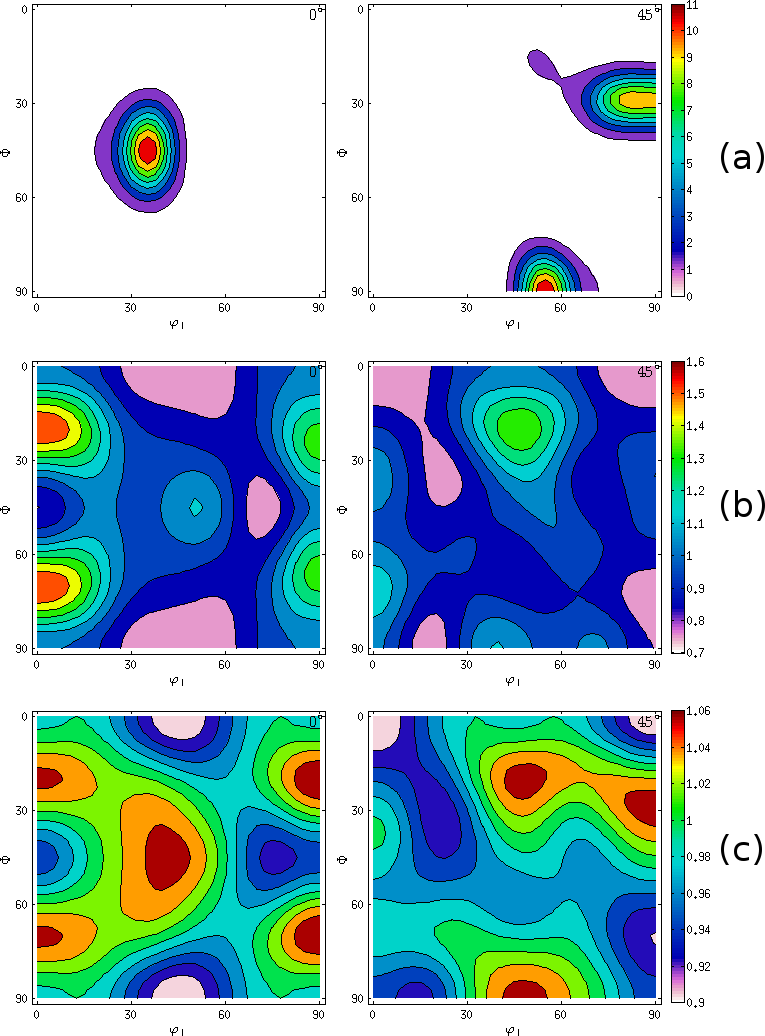
\includegraphics[width=\textwidth]{MicrovsODF_AlL}
  \caption{Size y strain vs ODF $Al_L$.}
  \label{fig:AlLMicro}
\end{figure}

\newpage
\section{Estudio de la microestructura por EBSD - Revisión}\label{S:AlEBSD}
\section{Discusión de resultados}\label{S:AlDis}
\section{Conclusiones}\label{S:AlConclusiones}
